\documentclass[10pt, a4paper]{report}
\usepackage[utf8]{inputenc}
\usepackage{amsfonts}
\usepackage{amsmath}
\usepackage{amssymb}
\usepackage{amsthm}
\usepackage[all,cmtip]{xy}
\usepackage{hyperref}
\usepackage[top=3cm, left=3cm,right=3cm, bottom=3cm]{geometry}
\usepackage{graphicx}
%\usepackage{subfig}
%\usepackage{subfigure}
\usepackage{caption}
\usepackage{subcaption}
\usepackage{float}
\usepackage{tikzsymbols}
\usepackage{algorithm}
\usepackage{mathtools}
\usepackage[noend]{algpseudocode}
\newcommand{\E}[0]{\mathbb{E}}
\newcommand{\Ll}[0]{\mathbb{L}}
\newcommand{\R}[0]{\mathbb{R}}
\newcommand{\Pp}[0]{\mathbb{P}}
\newcommand{\p}[0]{\mathfrak{p}}
\newcommand{\I}[0]{\mathcal{I}}
\newcommand{\F}[0]{\mathcal{F}}
\newcommand{\vv}[0]{\mathbf{v}}
\theoremstyle{definition}
\newtheorem{theorem}{Theorem}
\newtheorem{prop}{Proposition}
\newtheorem{lemma}{Lemma}
\newtheorem{coro}{Corollary}
\newtheorem{definition}{Definition}
\theoremstyle{remark}
\newtheorem{rmk}{Remark}
\newtheorem{ex}{Example}






\begin{document}
\begin{titlepage}
	\centering
	
\includegraphics[width=0.6\textwidth]{EPFL-Logo}\par\vspace{1cm}
	%{\scshape\LARGE École polytechnique fédérale de Lausanne \par}
	\vspace{1cm}
	{\scshape\Large Master thesis\par}
	\vspace{1.5cm}
	\hrulefill \\
	{\huge\bfseries A probabilistic approach to the classification of censored functional data \par}
	\hrulefill \\
	\vspace{2cm}
	{\Large William \textsc{Borgeaud dit Avocat}\par}
	\vfill
	{\Large
	supervised by\par
	Prof.~Victor \textsc{Panaretos}}
	
	\vfill
	
	% Bottom of the page
	{\large \today\par}
\end{titlepage}

\tableofcontents

\chapter{Introduction to Functional Data Analysis}
\section{What are functional data?}
\subsection{Explain the structure of functional data, the spaces they live in, expectation, covariance, observable discretized versions. }
\section{Statistical analysis of functional data}
\subsection{Explain the basic principles of estimation of mean and covariance with convergence rates, etc.. Also mention smoothing methods. }

\chapter{Censored functional data}
\section{Functional fragments framework}\label{introfrag}
\subsection{Explain the functional fragments framework and and the methods used by Kraus and Delaigle and Hall}
\textit{Censored functional data} or \textit{functional fragments} are functional data that are not observed in the full domain on which they are defined. If the data live in $\Ll^2(\mathcal{I})$ for some interval $\mathcal{I} \subset \R$, an example of functional fragment is a function $f \in \Ll^2(\mathcal{J})$ for some interval $\mathcal{J}\subset \mathcal{I}$.

By the \textit{functional fragments framework}, we mean the statistical framework in which some or all of the observed data are in the form of fragments of some underlying, unobservable, functional data. In this case, the data at hand are pairs $\{(X_i,\mathcal{O}_i)\}_{i=1}^n$, where the $X_i$'s are random functions in $\Ll(\mathcal{O}_i)$ for some subintervals $\mathcal{O}_i$. We will often assume that the subintervals $\{\mathcal{O}_i\}_{i=1}^n$ are themselves random, in order to make the asymptotic theory more tractable. This framework often arises in practice when an observation is unavailable before or after a certain time.\\
The main issue in the functional fragments framework is to know to what extent one can recover precise information on the underlying population from the observed fragments. For example, how precisely can we estimate the mean and covariance when no curve is fully observed.\\
Following \cite{DP2}, we distinguish between two ways in which the intervals $\{\mathcal{O}_i\}_{i=1}^n$ are distributed, see Figure \ref{fig:exfrags}:\\

\noindent
\textbf{1.} A ``blanket '' regime, where the curves are typically observed on most or all of the domain. Then the number of observations at a given point of the domain is close to the total number of observations.\\
\textbf{2.} A ``banded'' regime, where the lengths of the $\mathcal{O}_i$ are bounded by some value $\delta>0$. Then, we have no explicit information on the covariance of points that are at distance larger than $\delta$.
\begin{figure}[ht]
	\centering
	\begin{subfigure}{.3\textwidth}
		\centering
		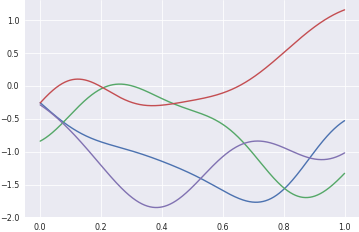
\includegraphics[width=.8\linewidth]{Code/images/21/full}
		\caption{Full curves}
	\end{subfigure}%
	\begin{subfigure}{.3\textwidth}
		\centering
		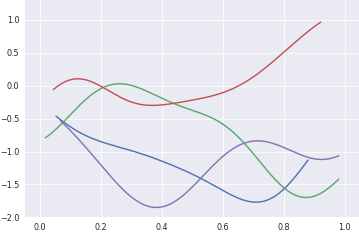
\includegraphics[width=.8\linewidth]{Code/images/21/blanket}
		\caption{\centering Fragments in the blanket regime}
	\end{subfigure}
	\begin{subfigure}{.3\textwidth}
		\centering
		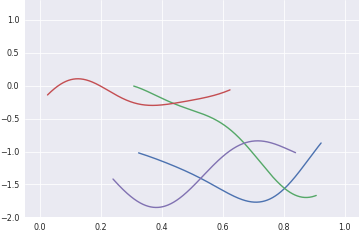
\includegraphics[width=.8\linewidth]{Code/images/21/frags}
		\caption{\centering Fragments in the banded regime}
	\end{subfigure}
	\caption{Example of functional fragments}
	\label{fig:exfrags}
\end{figure}

In the rest of this chapter, we will present various methods used in the literature dealing with those issues. 	

\section{Naive estimations}	
We present here the methods presented in \cite{Kraus1}. The data are i.i.d curves $X_i$ in $\Ll^2[0,1]$ observed only on a random interval $\mathcal{O}_i \subset [0,1]$, $i=1,...,n$. To estimate the population mean $\mu = \E[X_1]$ and covariance operator $\mathcal{K} = \E[(X_1-\mu) \otimes (X_1-\mu)]$, the unobserved parts of the curves are ignored and the sample estimators are created naively as follows. The sample mean $\hat{\mu}$ is found by taking the mean of the pointwise observed values: 
\[\hat{\mu}(t) = \frac{\mathbf{1}[\exists \mathcal{O}_i \ni t ]}{\sum_{i=1}^n \mathbf{1}[t \in \mathcal{O}_i]} \sum_{i=1}^n \mathbf{1}[t \in \mathcal{O}_i] \cdot X_i(t). \]
The covariance operator is estimated in the same fashion via its associated covariance kernel $K(\cdot,\cdot)$. The sample kernel is given by:
\[\hat{K}(s,t) = \frac{\mathbf{1}[\exists \mathcal{O}_i \ni s,t ]}{\sum_{i=1}^n \mathbf{1}[s,t \in \mathcal{O}_i]} \sum_{i=1}^n \mathbf{1}[s,t \in \mathcal{O}_i] \cdot \left\{X_i(s)-\hat{\mu}_{st}(s)\right\}\left\{X_i(t)-\hat{\mu}_{st}(t)\right\}, \]
where  $\hat{\mu}_{st}$ is an estimation of the mean using only the curves observed at $s$ and $t$:
\[\hat{\mu}_{st}(s) = \frac{\mathbf{1}[\exists \mathcal{O}_i \ni s,t ]}{\sum_{i=1}^n \mathbf{1}[s,t \in \mathcal{O}_i]} \sum_{i=1}^n \mathbf{1}[s,t \in \mathcal{O}_i] \cdot X_i(s). \]
The sample covariance operator $\hat{\mathcal{K}}$ is then defined by 
\[\hat{\mathcal{K}}f(t) = \int_{0}^{1} \! \hat{K}(s,t)f(s) \, \mathrm{d}s.\]
We note that this operator need not be positive-definite. This can be dealt with by clipping the negative eigenvalues to zero.\\
The following proposition, proved in \cite[Prop. \!1]{Kraus1}, shows that under some assumptions on the random intervals $\{\mathcal{O}_i\}_{i=1}^n$, the above estimates enjoy the same asymptotic convergence rate as their counterparts when the curves are fully observed.
\begin{prop}
	\begin{itemize}
		\item[]
		\item[1.] Suppose that $\mathbb{E}\Vert X_1\Vert^2<\infty$ and the $\mathcal{O}_i$'s are i.i.d with $\inf_{t \in [0,1]} \Pp\left[t \in \mathcal{O}_1\right]>0$. Then 
		\[\mathbb{E}\Vert \hat{\mu}-\mu\Vert^2 = O(n^{-1}) \text{ as } n \to \infty. \]
		\item[2.] Suppose further that $\mathbb{E}\Vert X_1\Vert^4<\infty$ and that $\inf_{s,t \in [0,1]} \Pp\left[s,t \in \mathcal{O}_1\right]>0$. Then 
		\[\mathbb{E}\Vert \hat{\mathcal{K}}-\mathcal{K}\Vert^2_{HS} = O(n^{-1}) \text{ as } n \to \infty. \]
	\end{itemize}
	\qed
\end{prop}
For the covariance operator, even though the theoretical convergence rate is good, in practice the estimate is not adequate in the ``banded'' regime (see Section \ref{introfrag}). The problem is that in this regime, the estimated kernel is necessarily zero in the region $\{(s,t)\in [0,1]^2 \, \mid \, \vert s-t\vert > \delta \}$. This problem that is not present in the ``blanket'' regime, as soon as one full curve is observed, see Figure .
\begin{figure}[H]
	\centering
	\begin{subfigure}{.3\textwidth}
		\centering
		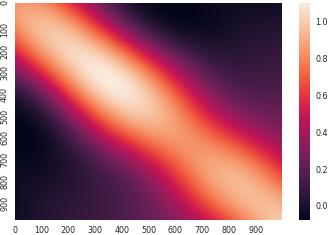
\includegraphics[width=.8\linewidth]{Code/images/22/truecov}
		\caption{Full curves}
	\end{subfigure}%
	\begin{subfigure}{.3\textwidth}
		\centering
		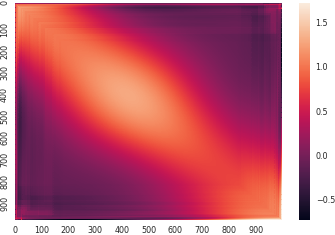
\includegraphics[width=.8\linewidth]{Code/images/22/blanketheat}
		\caption{\centering Fragments in the blanket regime}
	\end{subfigure}
	\begin{subfigure}{.3\textwidth}
		\centering
		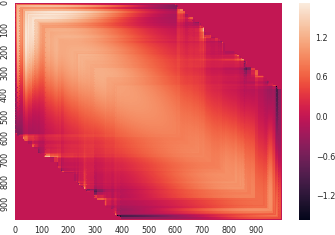
\includegraphics[width=.8\linewidth]{Code/images/22/fragsheat}
		\caption{\centering Fragments in the banded regime}
	\end{subfigure}
	\caption{Sample estimates of the covariance kernel in the different regimes}
	\label{fig:excov}
\end{figure}

\section{Curve extension}
In \cite{DH1}, the authors take the approach of manually extend the fragments by gluing some of their parts. This procedure is carried on in the context of classification, but it can readily be expended to the plain estimation of the population mean and covariance.\\
The extension of a fragment to the right is done by iteratively gluing a small section of another randomly chosen nearby fragment to the right endpoint of the original fragment. Likewise for the extension to the left. A few steps of this procedure are shown in Figure \ref{fig:gluingsteps}.
\begin{figure}[htp]
	\centering
	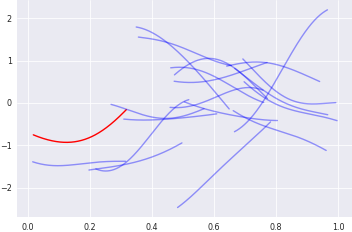
\includegraphics[width=.4\textwidth]{Code/images/23/step1}\quad
	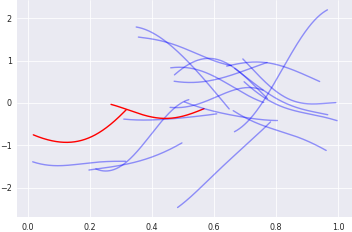
\includegraphics[width=.4\textwidth]{Code/images/23/step2}\quad
	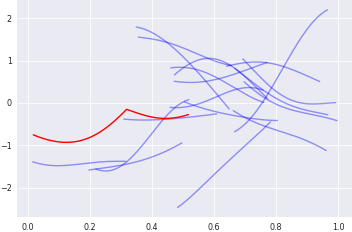
\includegraphics[width=.4\textwidth]{Code/images/23/step3}
	
	\medskip
	
	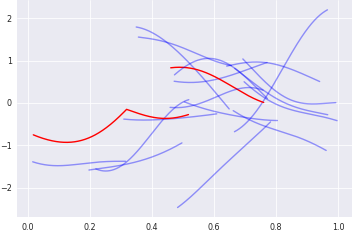
\includegraphics[width=.4\textwidth]{Code/images/23/step4}\quad
	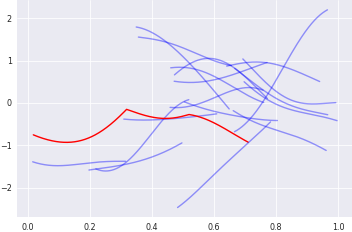
\includegraphics[width=.4\textwidth]{Code/images/23/step5}
	
	\caption{Illustration of a few steps of the gluing procedure}
	\label{fig:gluingsteps}
\end{figure}

In this way, for each fragment $(X_i, \mathcal{O}_i)$, one gets a curve $\tilde{X}_i$ defined on the entire domain. From these full curves, the sample mean and covariance can be estimated. This estimation method works both in the ``blanket'' and the ``banded'' regime, since in both cases full curves are constructed. Examples of those estimates are shown in Figure \ref{fig:gluingex}.
\begin{figure}[H]
	\centering
	\begin{subfigure}{.4\textwidth}
		\centering
		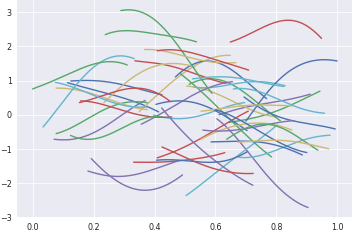
\includegraphics[width=.8\linewidth]{Code/images/23/frags}
		\caption{Fragments}
	\end{subfigure}%
	\begin{subfigure}{.4\textwidth}
		\centering
		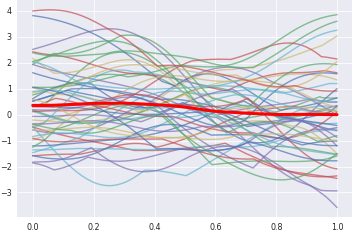
\includegraphics[width=.8\linewidth]{Code/images/23/extended}
		\caption{\centering Reconstructed curves with their mean in red}
	\end{subfigure}
	
	
	\medskip
	
	
	\begin{subfigure}{.4\textwidth}
		\centering
		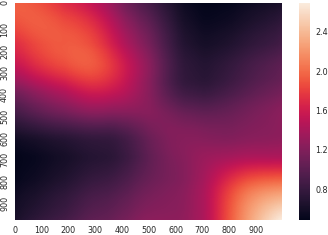
\includegraphics[width=.8\linewidth]{Code/images/23/cov}
		\caption{\centering Estimated covariance kernel form the reconstructed curves }
	\end{subfigure}
	\caption{Example of mean and covariance estimation using the gluing procedure}
	\label{fig:gluingex}
\end{figure}



\section{Covariance recovery}
\subsection{Explain the method by Descary and Panaretos to recover the covariance from functional fragments}

\chapter{Gaussian measures in Hilbert space}
\section{Gaussian measures in finite dimensions}
\subsection{Basic definitions}
\section{Gaussian measures in infinite dimensions}
\subsection{Definition and construction of gaussian measures in infinite dimensions. Basic properties.}
\section{The Feldman-Hajek theorem}
\subsection{Stating the F-H theorem with some intuition}

\chapter{Classification of functional data}
\section{Linear and quadratic discriminant analysis for functional data}
\subsection{Explain LDA and QDA}
\section{Classification of functional fragments}
\subsection{Explain the work done by Kraus and Delaigle and Hall on the classification of functional fragments and my work}
\section{A probabilistic approach to classification}
\subsection{Explain the perfect classification phenomenon through the F-H theorem. If I manage to find something, also the classification of fragments.}

\chapter{Numerical experiments}









\bibliography{biblio} 
\bibliographystyle{apalike}


%\begin{thebibliography}{1}
%	
%	\bibitem{pana} Marie-Hélène Descary, Victor M. Panaretos {\em Recovering Covariance from Functional Fragments}  2017	.
%	
%\end{thebibliography}


\end{document}